\documentclass{beamer}
%
% Choose how your presentation looks.
%
% For more themes, color themes and font themes, see:
% http://deic.uab.es/~iblanes/beamer_gallery/index_by_theme.html
%
\mode<presentation>
{
  \usetheme{Dresden}      % or try Darmstadt, Madrid, Warsaw, ...
  \usecolortheme{orchid} % or try albatross, beaver, crane, ...
  \usefonttheme{default}  % or try serif, structurebold, ...
  \setbeamertemplate{navigation symbols}{}
  \setbeamertemplate{caption}[numbered]
} 


\newcommand{\tn}{\textnormal}
\newcommand{\Ehigh}{\mathcal{E}^\tn{high}_i}
\newcommand{\Emed}{\mathcal{E}^\tn{med}_i}
\newcommand{\NN}{\mathcal{N}}

\usepackage{amsmath,amssymb,amsfonts}
\usepackage{mathpazo}
\usepackage{graphicx,tabularx,epsfig}
\usepackage[english]{babel}
\usepackage[utf8x]{inputenc}
\usepackage{booktabs}
\usepackage{xcolor}
\usepackage{multirow}
\usepackage{subfig}
\usepackage{booktabs}
\usepackage{lmodern}% http://ctan.org/pkg/lm

\definecolor{adired}{rgb}{0.83, 0.00, 0.00}
\definecolor{adiblue}{rgb}{0.19, 0.361, 0.769}
\definecolor{adigreen}{rgb}{0.012, 0.561, 0.180}

% *** Presentation to seminar (2018+) ***

\title[Robustness in Power Grid Planning]{Robustness in Power Grid Expansion Planning}
\author[Sarid, Tzur]{Adi Sarid, Michal Tzur}
\institute[Tel-Aviv University]{\normalsize Department of Industrial Engineering, Tel-Aviv University, Israel}
\date{December 31st, 2018}

\titlegraphic{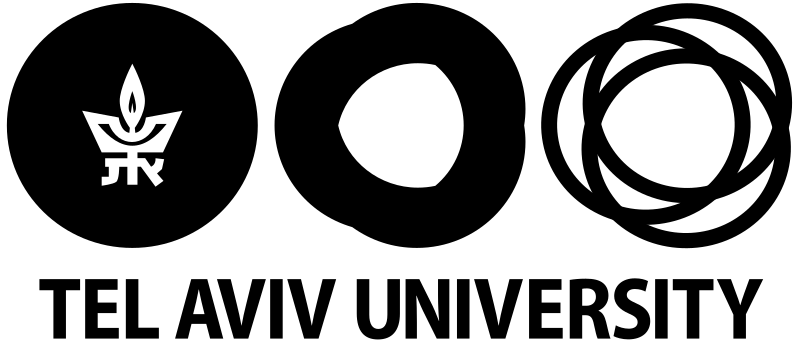
\includegraphics[width=2.5cm]{Aux_files/Tel_Aviv_university_logo.png}}
\begin{document}

\begin{frame}
  \titlepage
\end{frame}

\addtobeamertemplate{navigation symbols}{}{%
    \usebeamerfont{footline}%
    \usebeamercolor[fg]{footline}%
    \hspace{1em}%
    \insertframenumber/\inserttotalframenumber
}

\section{Introduction}
\subsection{Background}
\begin{frame}
\frametitle{Why Should We Care About Power Grid ``Robustness''}
\begin{itemize}
	\item Each year, weather related outages in the US incur an average cost of \$18-\$33 billion [1]
	\item The grid is also vulnerable to a variety of threats other than weather (cyber, terror, natural disasters, etc.)
	\item The grid is a \textbf{critical infrastructure}
	\item Disruptions cannot be totally avoided, but they can be mitigated
	\begin{itemize}
		\item Infrastructure \textbf{design} (e.g., capacity upgrades, micro-grids, DG)
		\item \textbf{Realtime} mitigation (e.g., islanding, restoration)
	\end{itemize}
  \item How can we design more robust power grids?
\end{itemize}
\vspace{0.2in}
\tiny [1] President's Council of Economic Advisers and the U.S. Department of Energy, Economic benefits of increasing electric grid resilience to weather outages, 2013.
\end{frame}

\begin{frame}
\frametitle{What is Robustness?}
\begin{block}{Robustness \small[2]}
\begin{itemize}
	\item Robustness is related to \emph{how much} damage occurs as a consequence of an unexpected perturbation. \pause 
    \item The greater the damage, the system is less robust. For example:
	\begin{itemize}
		\item Expected loss of load (electricity)
		\item Probability for loss of load (of a certain amount)
	\end{itemize} %\pause
	%\item Resilience measures \emph{how quickly} the network can retrieve from such damage. \pause For example:
	%\begin{itemize}
		%\item The expected time it takes to restore electricity supply
	%\end{itemize}
\end{itemize}
\end{block}
\vspace{0.2in}
\tiny [2] Cuadra \emph{et al.}, A critical review of robustness in power grids using complex networks concepts. \emph{Energies}, 2015.
\end{frame}

%\subsection{Related Work}
%\begin{frame}
%\frametitle{Related Work -- TBD}
%\begin{itemize}
	%\item Measure definitions (robustness/resilience)
	%\item Design decisions
	%\item Grid restoration
	%\item Models of cascades
	%\item Flow models (AV vs. DC)
	%\item Solution methods
	%\begin{itemize}
		%\item Heuristics
		%\item Linear programming
	%\end{itemize}
%\end{itemize}
%\end{frame}

\section{Power Flow}
\subsection{Layers of the grid and the DC load flow model}
\begin{frame}
\frametitle{Layers of the Grid}
\framesubtitle{Generation, transmission, and distribution}
\begin{figure}[h]
		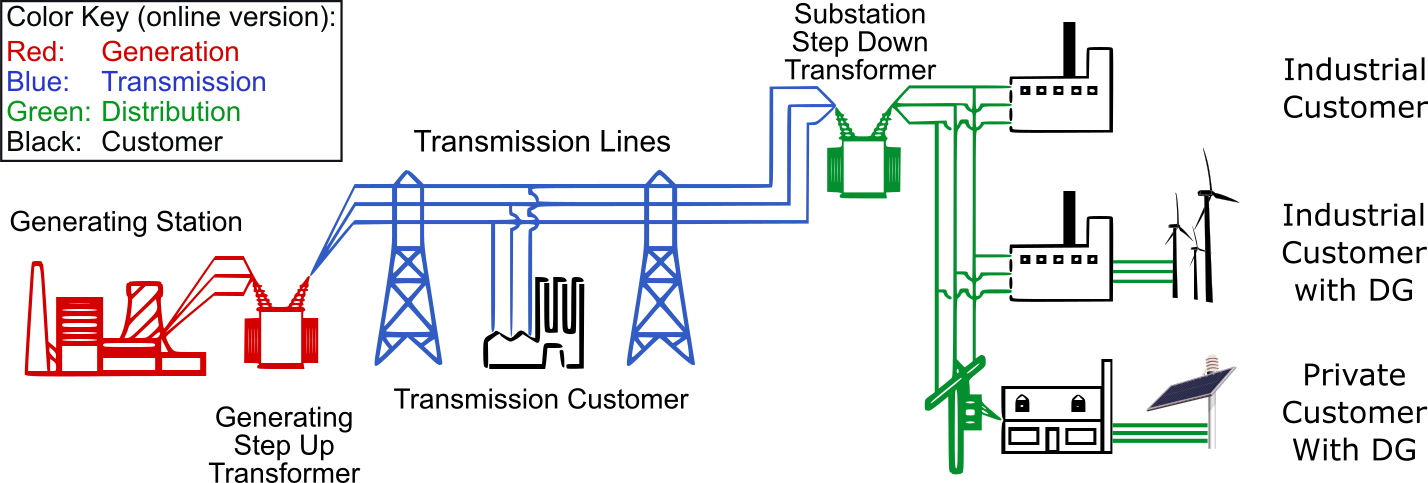
\includegraphics[width=0.5\textwidth]{Aux_files/figure_1_Electricity_grid_simple_North_America.png}
	\label{fig:figure_1_Electricity_grid_simple_North_America}
\end{figure}
\pause
\footnotesize Eventually the layers are arranged into a network. The following illustrates the generation and transmission layers:
\vspace{-0.1in}
\begin{figure}
		%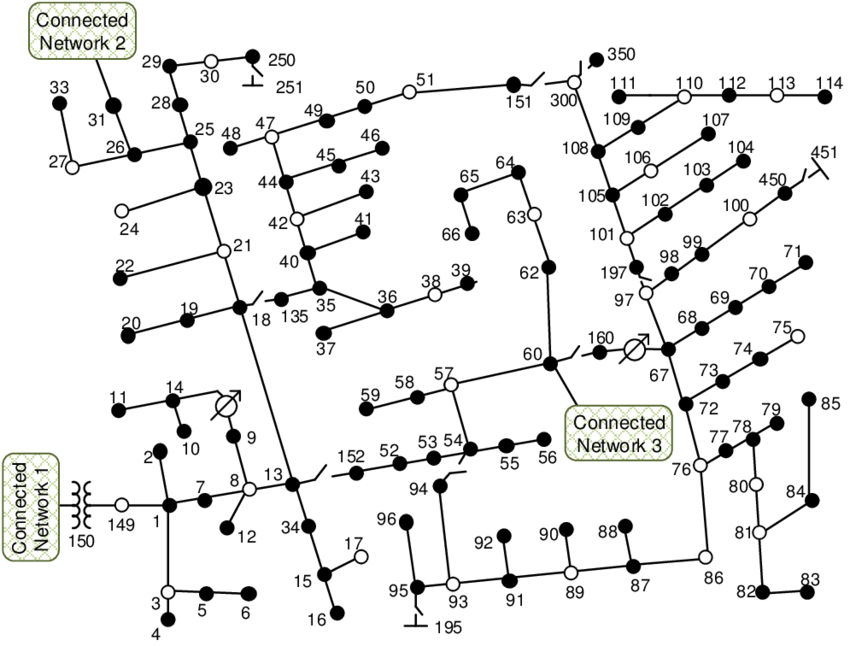
\includegraphics[width=.35\textwidth]{Aux_files/figure_2_alternative_example_ieee123_mod.png}
		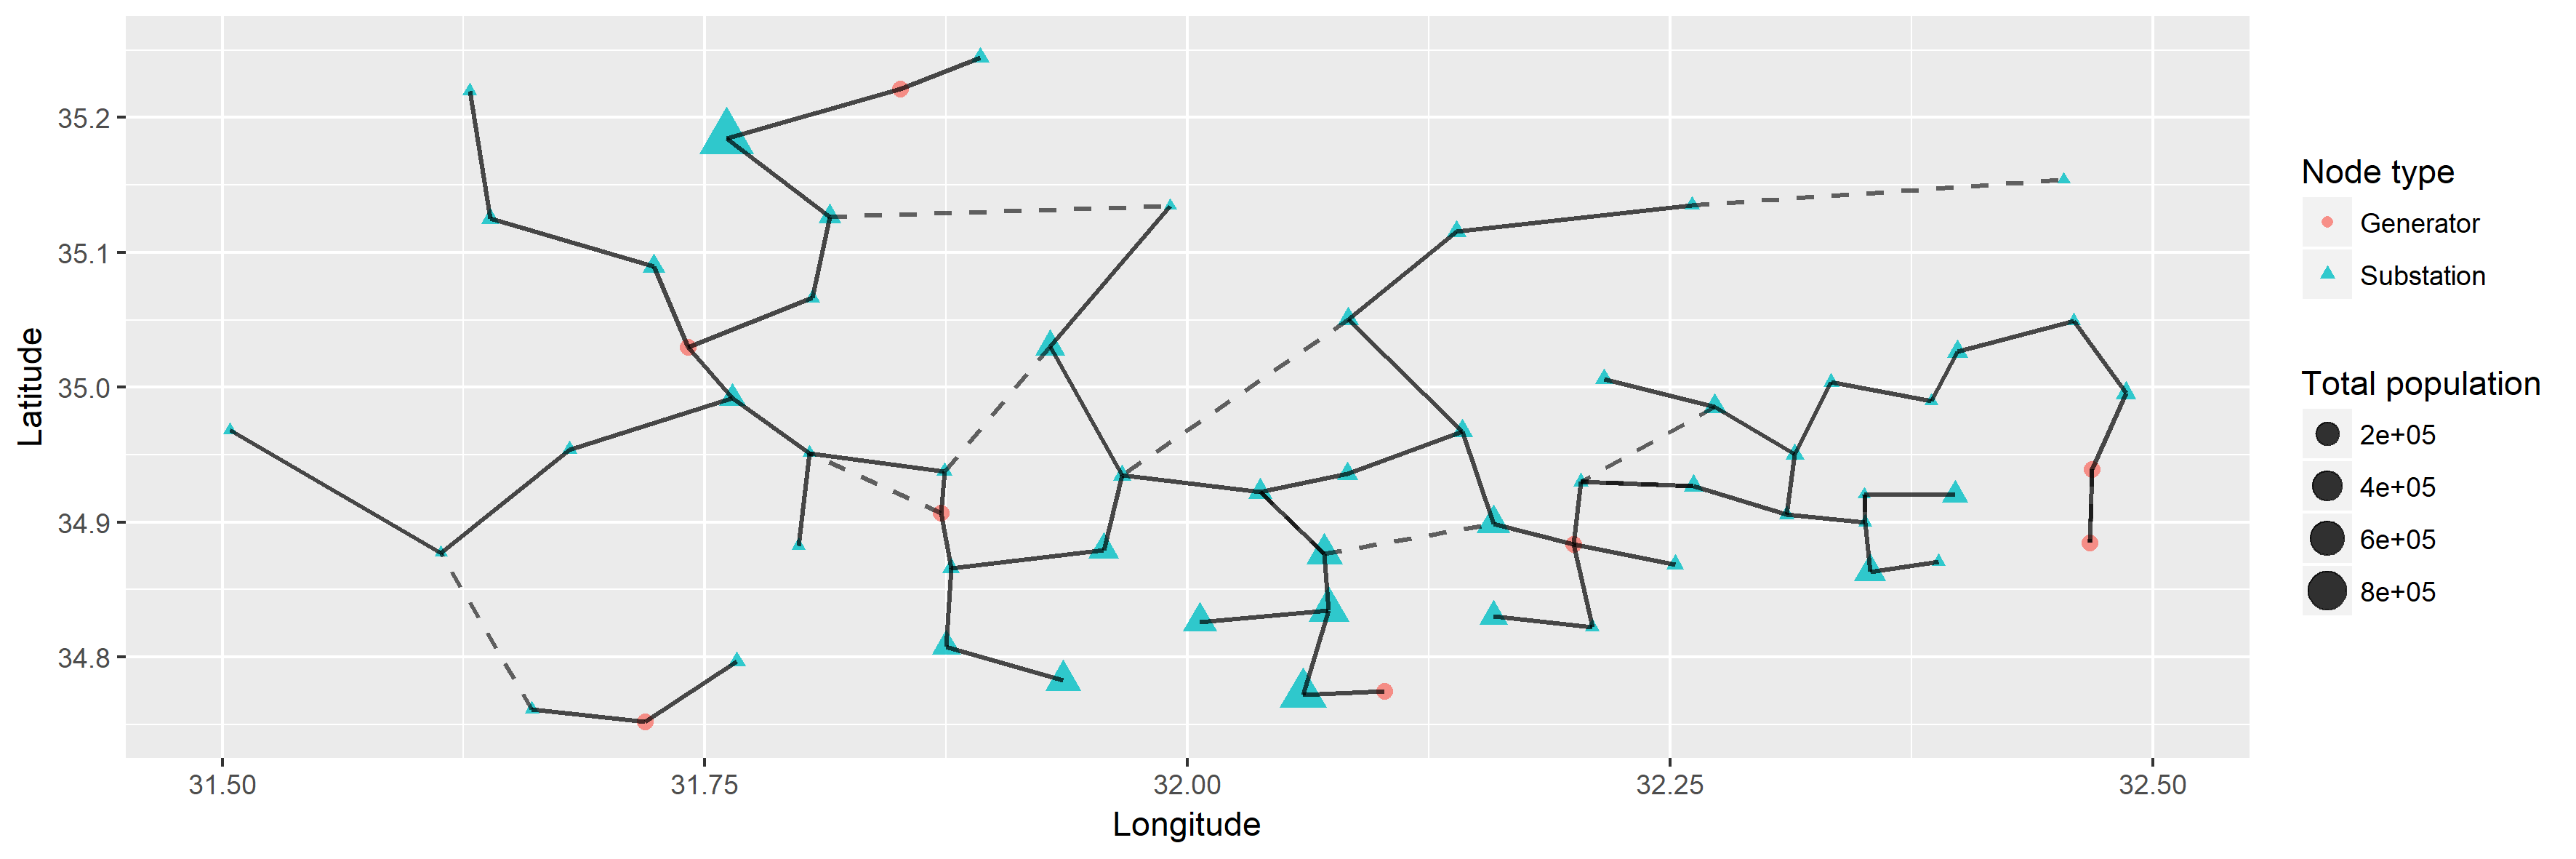
\includegraphics[width=1\textwidth]{Aux_files/figure_2_example_grid.png}
	\label{fig:figure_2_example_grid}
\end{figure}
\end{frame}

% \begin{frame}
% \frametitle{The Flow Equations}\footnotesize
% Two popular models of flow:
% \begin{itemize}
% 	\item AC load flow (alternating current) -- Non linear, used for realtime problems (sometimes in planning)
% 	\item \textbf{DC load flow (direct current)} -- Linear, used as an approximation to AC in infrastructure design problems [3]
% \end{itemize}\pause
% The DC load flow equations:
% \begin{align*}
% 	\sum_j{f_{ij}} = d_i & \quad\forall i\in\mathcal{N}, \{i,j\}\in\mathcal{L}\\
% 	\theta_i-\theta_j-x_{ij}f_{ij}=0 & \quad\forall \{i,j\}\in\mathcal{L}
% \end{align*}\pause

% \tiny [3] Bienstock, Daniel and Mattia, Sara, Using mixed-integer programming to solve power grid blackout problems, \emph{Discrete Optimization}, 2007.
% \end{frame}

\begin{frame}
\frametitle{The Flow Equations}\footnotesize
The DC load flow equations:
\begin{align*}
	\sum_j{f_{ji}} = d_i & \quad\forall i\in\mathcal{N}, \{i,j\}\in\mathcal{L}\\
	\theta_i-\theta_j-x_{ij}f_{ij}=0 & \quad\forall \{i,j\}\in\mathcal{L}
\end{align*}
Flow preservation + Active power (phase angle constraints), where:
\begin{itemize}
	\item Decision variables: $f_{ij}=$ flow in $\{i,j\}$; \ $\theta_i=$ phase angle at $i$
	\item Parameters: $x_{ij}=$ reactance of $\{i,j\}$; \ $d_i=$ demand (supply) at $i$
\end{itemize}

\begin{block}{\small Lemma 1. Flow solution uniqueness}
If the flow preservation and active power constraints have a solution, then this solution is unique in the $f_{ij}$ variables.
\end{block}
Proof sketch. For trees, the flow can be determined incrementally, by traversing the nodes. For a graph with cycles it requires a bit more work but still holds (can be proved by contradiction).
\end{frame}

\subsection{Cascade Failure Mechanism}
\begin{frame}
\frametitle{What is a ``Cascading Failure''?}\small
The DC load flow model does not include line capacities, however, a transmission line cannot conduct infinite power. Hence, the power grid is vulnerable to a failure process, as follows:
\begin{enumerate}
  \item<1->An external factor (e.g, extreme weather) causes a certain failure
	\item<2->The current is immediately rerouted (by the physical laws of flow)
	\item<3->If the current of a transmission line then exceeds a threshold, the line overheats and breaks
	\item<4->When a line breaks, the current is again rerouted (by physical laws)
	\item<5->This process continues on until no line exceeds its capacity threshold
\end{enumerate}
\begin{itemize}
	\item<6->The cascade process is usually described via a simulation model [3,4]
\end{itemize}

\uncover<6->{
\tiny [3] Bienstock, Daniel and Mattia, Sara, Using mixed-integer programming to solve power grid blackout problems, \emph{Discrete Optimization}, 2007.\\\tiny[4] Soltan \emph{et. al.}, Cascading failures in power grids: analysis and algorithms, \emph{Proceedings of the 5th international conference on Future energy systems}, 2014.}
\end{frame}

\begin{frame}
\frametitle{Example of a Cascade}
\begin{itemize}
	\item Node $i$ with demand $d_i$
	\item Edge $\{G,i\}$ with capacity $d_i+\epsilon$
	\item Edges $\{1,2\}, \{2,3\}$ with ``infinite'' (very large) capacity
	%\item Reactance $(d_3+\epsilon)x_{G3}=\epsilon x_{23} + (d_1+d_2-\epsilon)x_{G2}$
\end{itemize}
%\vspace{-0.2in}
%\begin{figure}
	%\centering
	  %\setcounter{subfigure}{0}% Reset subfigure counter to avoide beamer \pause counter clash
		%\subfloat[Nominal]{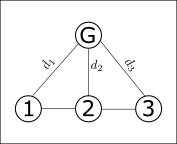
\includegraphics[width=0.23\textwidth]{Aux_files/figure_3_a_cascade_example.png}}
		%\pause
		%%\hspace{0.1in}
		%\subfloat[Init fail]{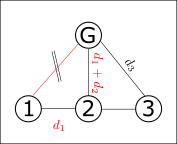
\includegraphics[width=0.23\textwidth]{Aux_files/figure_3_b_cascade_example.png}}%\hspace{0.1in}
		%\pause
		%\subfloat[Cascade \#1]{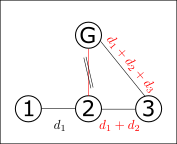
\includegraphics[width=0.23\textwidth]{Aux_files/figure_3_c_cascade_example.png}}%\hspace{0.1in}
		%\pause
		%\subfloat[Cascade \#2]{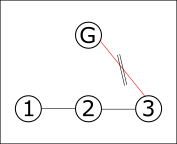
\includegraphics[width=0.23\textwidth]{Aux_files/figure_3_d_cascade_example.png}}
%\end{figure}

\begin{figure}
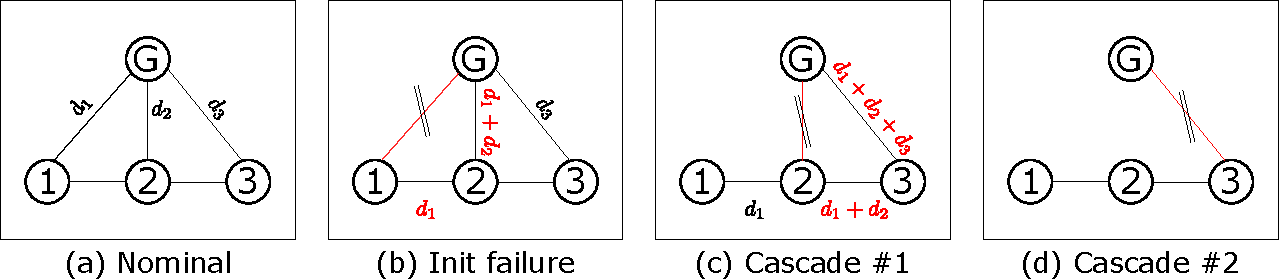
\includegraphics[width=1\textwidth]{Aux_files/figure_3_full.pdf}
\end{figure}

\begin{itemize}
	\pause\item This grid completely fails, no consumer is supplied
	\pause\item If edge $\{1,2\}$ hadn't existed, consumers $2,3$ would have remained with power supply
\end{itemize}

\pause ``\textbf{Braess's paradox} in power grids''...
\end{frame}

% should include a toy example
% should include conditions for one casecade depth, N-cascade depth

\section{Design for Robustness}
% I would not discuss a characterization of 1-cascade depth due to lack of time
%\subsection{Na\"{i}ve Characterization of 1-cascade depth}
% What do we measure?
\subsection{Single Cascade}\footnotesize
\begin{frame}
\frametitle{Design for Robustness}
Design a power grid with \textbf{minimum loss of load} subject to:
\begin{itemize}
	\item Failure scenarios (scenarios which describe failures due to external factors)
	\item Considering cascade outcomes due to initial failures
	\item Using the DC load flow model
	\item Limited budget
\end{itemize}\pause
Decision variables:
\begin{itemize}
	\item Upgrade capacity of transmission lines (edges)
	\item Establish new transmission lines
	\item Establish units with backup capacity at consumer nodes (DG or battery)
	\item Generation and flow variables
\end{itemize}\pause
Start simple -- assume up to a single cascade:
\begin{enumerate}
  \setcounter{enumi}{-1}
	\item Initial failure;
	\item Flow after failure, which causes a cascade; 
	\item After cascade flow rearranges again and no further cascades
\end{enumerate}
\end{frame}

% a MILP for one cascade depth
\begin{frame}
\frametitle{Design for Robustness -- 1-cascade depth}
\framesubtitle{What happens if only a single cascade may occur?}
\vspace{0.1in}
Minimum expected loss of load:
\begin{align*}
\sum_{s\in\mathcal{S}}{p_s}\sum_{i\in\mathcal{N}\setminus\{G\}}{\left(d_i-w_i^{2,s}\right)}	
\end{align*}
\footnotesize
Variable domain:
\begin{align*}
	 \forall i,j\in\mathcal{N}, t\in\{1,2\}, s\in\mathcal{S}:\\
	 g_i^s, w_i^{t,s}, c_{ij}^l, c_i^g\geq0\\
	 F_{ij}^s, Z_i\in\{0,1\}\\
	 \forall (i,j)\in\mathcal{L}^e:\\
	 X_{ij} \in\{0,1\}
\end{align*}
Investment cost constraint (budget):
\begin{align*}
	 \sum_{(i,j)\in\mathcal{L}}{h_{ij}c_{ij}^l} + \sum_{i\in\mathcal{N}}\left(h_ic_i^g + H_iZ_i\right) + \sum_{(i,j)\in\mathcal{L}^e}{H_{ij}X_{ij}} \leq C
\end{align*}
\end{frame}
\begin{frame}
\frametitle{Design for Robustness -- 1-cascade depth -- cont.}\footnotesize
Conservation of flow (the DC load flow model, for $t=1$):
\begin{align*}
   \sum_{j\in\mathcal{N}|(j,i)\in\mathcal{L}\backslash\mathcal{F}^s}f_{ji}^{1,s}-\sum_{j\in\mathcal{N}|(i,j)\in\mathcal{L}\backslash\mathcal{F}^s}f_{ij}^{1,s} = d_i & \quad \forall i\in\mathcal{N}, s\in\mathcal{S}\\
	 \theta_i^{1,s}-\theta_j^{1,s}-x_{ij}f_{ij}^{1,s}=0 & \quad \forall (i,j)\in\mathcal{L}^0, (i,j)\notin\mathcal{F}^s, s\in\mathcal{S}\\
	 \color{red}{\theta_i^{1,s}-\theta_j^{1,s}-x_{ij}f_{ij}^{1,s}\leq M (1-X_{ij})} & \quad \forall (i,j)\in\mathcal{L}^e\backslash\mathcal{F}^s, s\in\mathcal{S}\\
	 \theta_i^{1,s}-\theta_j^{1,s}-x_{ij}f_{ij}^{1,s}\geq -M (1-X_{ij}) & \quad \forall (i,j)\in\mathcal{L}^e\backslash\mathcal{F}^s,  s\in\mathcal{S}
\end{align*}
Cascade effects which occur at $t=1$:
\begin{align*}
	\color{red}{f_{ij}^{1,s} \leq c_{ij}^0+c_{ij}^l + M\cdot F_{ij}^s} & \qquad \forall (i,j)\in\mathcal{L}\backslash\mathcal{F}^s, s\in\mathcal{S}\\
	 -f_{ij}^{1,s} \leq c_{ij}^0+c_{ij}^l + M\cdot F_{ij}^s & \qquad \forall (i,j)\in\mathcal{L}\backslash\mathcal{F}^s, s\in\mathcal{S}
\end{align*}
\end{frame}

\begin{frame}
\frametitle{Design for Robustness -- 1-cascade depth -- cont.}\footnotesize
Transmission capacity:
\begin{align*}
	 f_{ij}^{t,s} \leq M\cdot X_{ij} & \qquad \forall t\in\mathcal{T}, s\in\mathcal{S}, (i,j)\in\mathcal{L}^e\\
	 f_{ij}^{t,s} \geq -M\cdot X_{ij} & \qquad \forall t\in\mathcal{T}, s\in\mathcal{S}, (i,j)\in\mathcal{L}^e
\end{align*}
\begin{align*}
	 \color{red}{f_{ij}^{2,s} \leq M\cdot(1-F_{ij}^s)} & \qquad \forall (i,j)\in\mathcal{L}\backslash\mathcal{F}^s, s\in\mathcal{S}\\
	 f_{ij}^{2,s} \geq -M\cdot(1-F_{ij}^s) & \qquad \forall (i,j)\in\mathcal{L}\backslash\mathcal{F}^s, s\in\mathcal{S}
\end{align*}
Limit supply (do not exceed demand at $t=2$):
\begin{align*}
   \sum_{i\in\mathcal{N}}w_i^s = \sum_{i\in\mathcal{N}}g_i^s & \qquad \forall s\in\mathcal{S}\\
   w_i^{s} \leq d_i & \qquad \forall i\in\mathcal{N}\backslash\{G\}
\end{align*}
\end{frame}

\begin{frame}
\frametitle{Design for Robustness -- 1-cascade depth -- cont.}\footnotesize
Generation capacity:
\begin{align*}
	 g_i^{s} \leq c_i^g & \qquad \forall i\in\mathcal{N}, s\in\mathcal{S}\\
	 g_i^{s} \leq M\cdot Z_i & \qquad \quad\forall i\in\mathcal{N}
\end{align*}
Conservation of flow after cascade ($t=2$):
\begin{align*}
	 \sum_{(j,i)\in\mathcal{L}\backslash\mathcal{F}^s}f_{ji}^{2,s}-\sum_{(i,j)\in\mathcal{L}\backslash\mathcal{F}^s}f_{ij}^{2,s} + g_i^s - w_i^s = 0 & \qquad \forall i  \in\mathcal{N}, s\in\mathcal{S}\\
	 \theta_i^{2,s}-\theta_j^{2,s}-x_{ij}f_{ij}^{2,s}\leq M F_{ij}^s & \qquad \forall (i,j)\in\mathcal{L}^0\backslash\mathcal{F}^s, s\in\mathcal{S}\\
	 \theta_i^{2,s}-\theta_j^{2,s}-x_{ij}f_{ij}^{2,s}\geq -M F_{ij}^s & \qquad \forall (i,j)\in\mathcal{L}^0\backslash\mathcal{F}^s, s\in\mathcal{S}\\
	\theta_i^{2,s}-\theta_j^{2,s}-x_{ij}f_{ij}^{2,s}\leq M (1-X_{ij}) + M F_{ij}^s & \quad \forall (i,j)\in\mathcal{L}^e\backslash\mathcal{F}^s, s\in\mathcal{S}\\
	 \theta_i^{2,s}-\theta_j^{2,s}-x_{ij}f_{ij}^{2,s}\geq -M (1-X_{ij}) - M F_{ij}^s & \quad \forall (i,j)\in\mathcal{L}^e\backslash\mathcal{F}^s, s\in\mathcal{S}	
\end{align*}
\end{frame}

\subsection{Any number of cascades}
\begin{frame}
\frametitle{Consistency and Limitations}
\begin{block}{Theorem 1. Consistency}
The optimal solution is ``physically consistent'', i.e.:
\begin{enumerate}
\item The flow at $t=1$ ($f_{ij}^{1,s}$) is equal to the DC load flow solution for a power grid at step $t=1$;
\item The objective value (unsatisfied demand at step $t=2$) is equal to the unsatisfied demand which a DC load flow model yields (after the cascade)
\end{enumerate}
\end{block}\pause\small
Proof sketch
\begin{itemize}
	\item For $t=1$ the result is trivial thanks to the uniqueness of the DC load flow solution.
	\item For $t=2$, this is a bit trickier. We don't prove that the flow itself is consistent (it doesn't have to be), just that the objective is. This is done by contradiction.
\end{itemize}
\end{frame}

\begin{frame}
\frametitle{Characterization of grids with 1-depth cascades}
\begin{block}{Theorem 2. A sufficient condition for up to 1-depth cascades}
Let $s$ be a failure scenario. Let the path $p_1$ lead from a generator $G$ to a node $i$, and assume $p_1$ includes an edge which fails in scenario $s$. 

Let $p_2$ be another path to $i$ from any generator $G'$ (which survives the initial failure of $s$), and $j\in p_2$ (a node on $p_2$). 

Then, if there is no alternative path to $j$ other than the subset of $p_2$, the failure by scenario $s$ will not lead to more than 1 cascade step.\pause
\end{block}
This characterization can be easily illustrated \textcolor{red}{(the red arrow should not exist)}:
\begin{figure}%
\centering
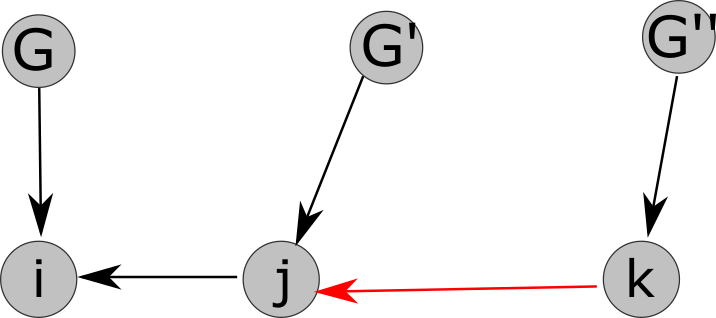
\includegraphics[width=0.4\textwidth]{Aux_files/characterization.png}
\end{figure}
What happens when we cannot guarantee a single cascade depth?
\end{frame}

\begin{frame}
\frametitle{What happens when we cannot guarantee a single cascade depth?}
\begin{itemize}
	\item Approach fails when trying a ``straightforward'' generalization of the optimization problem.
	\item The additional degrees of freedom (of generation variables) gives a solution which is not ``physically consistent''.
	\item Can be used with transmission line capacities as an approximation -- but how good would that approximation be? we'll see in a few slides.
\end{itemize}
\end{frame}


\begin{frame}
\frametitle{Second Approach ``Cascade Trees''}
If we could ``preprocess'' the solution tree and resulting cascades at each node, then we can essentially enumerate all possible failure combinations.
\begin{figure}[h]
	\centering
		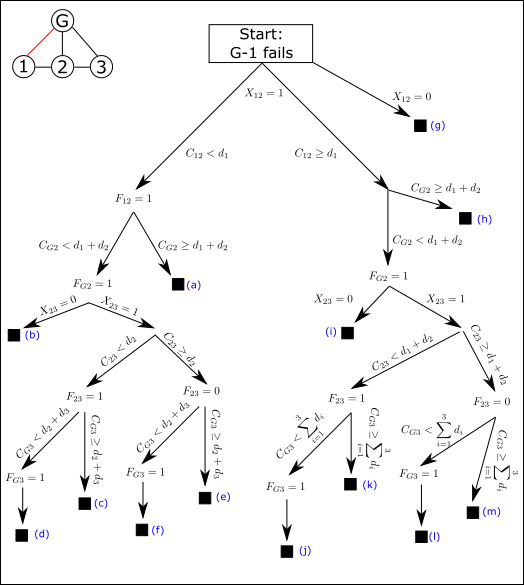
\includegraphics[width=0.30\textwidth]{Aux_files/figure_4_three-step-cascade-tree.png}
	\label{fig:figure_4_three-step-cascade-tree}
\end{figure}
Unfortunately, such preprocessing is too complex (too many options), but this can be generated \textbf{``on-the-fly''} using a \textbf{cutting plane} ``lazy'' constraints framework.
\end{frame}


\begin{frame}
\frametitle{Algorithm for an n-Cascade Depth Design Problem}
\small
%\only<2>{Solve an infrastructure design problem -- no casacde constraints}
%\only<3>{Check the the failures in solution vs. cascade simulation}
%\only<4>{If there are inconsistencies add them as new constraints and solve again}
\begin{figure}[h]
	\centering
		\includegraphics<1>[width=1\textwidth]{Aux_files/figure_5a_PGRO2_explained.pdf}
		\includegraphics<2>[width=1\textwidth]{Aux_files/figure_5b_PGRO2_explained.pdf}
		\includegraphics<3>[width=1\textwidth]{Aux_files/figure_5c_PGRO2_explained.pdf}
		\includegraphics<4->[width=1\textwidth]{Aux_files/figure_5d_PGRO2_explained.pdf}
	\label{fig:figure_5_PGRO2_algorithm}
\end{figure}
\begin{itemize}\footnotesize
	\item<5->Add-on: ``branching priorities'' -- save the failure variables ($F$) for last!
	\item<6->Heuristic callback: update incumbent solution during simulation step
\end{itemize}
\end{frame}

\subsubsection{Large Neighborhood Search}
\begin{frame}
\frametitle{Third Approach: a Large Neighborhood Search Heuristic (LNS)}
This meta-heuristic is based on ``destroying'' and ``rebuilding'' solutions. How does it work? (Pisinger, 2010)
\begin{itemize}
	\item start with a feasible solution $x$.
	\item \textbf{repeat}
	\begin{itemize}
		\item ``Destroy'' the solution $x$ (perturb the solution, until it is infeasible).
		\item ``Rebuild'' the infeasible solution back to a feasible solution $x'$.
		\item Check if $x'$ is better than $x$. If it is, update $x=x'$
	\end{itemize}
\item \textbf{until} stop criterion is met
\item \textbf{return }$x$
\end{itemize}
In our case, destroying the solution is upgrading the grid slightly above budget, and repairing the solution is giving up on some upgrades to converge back to budget.
\end{frame}
% cascade tree illustration for more complex cases
% the lazy constraints algorithm

\section{Results}
\subsection{Percent supplied}
\begin{frame}
\frametitle{Results -- percent supplied per instance}
\framesubtitle{Experiment based on four IEEE grids (30, 57, 118, and 300 nodes).}
\tiny
\begin{itemize}
	\item Two possible budgets ($30\%$ and $50\%$ of max expanse).
	\item Two initial capacity settings ($5\%$ and $20\%$ above nominal flow).
\end{itemize}
\begin{figure}
\centering
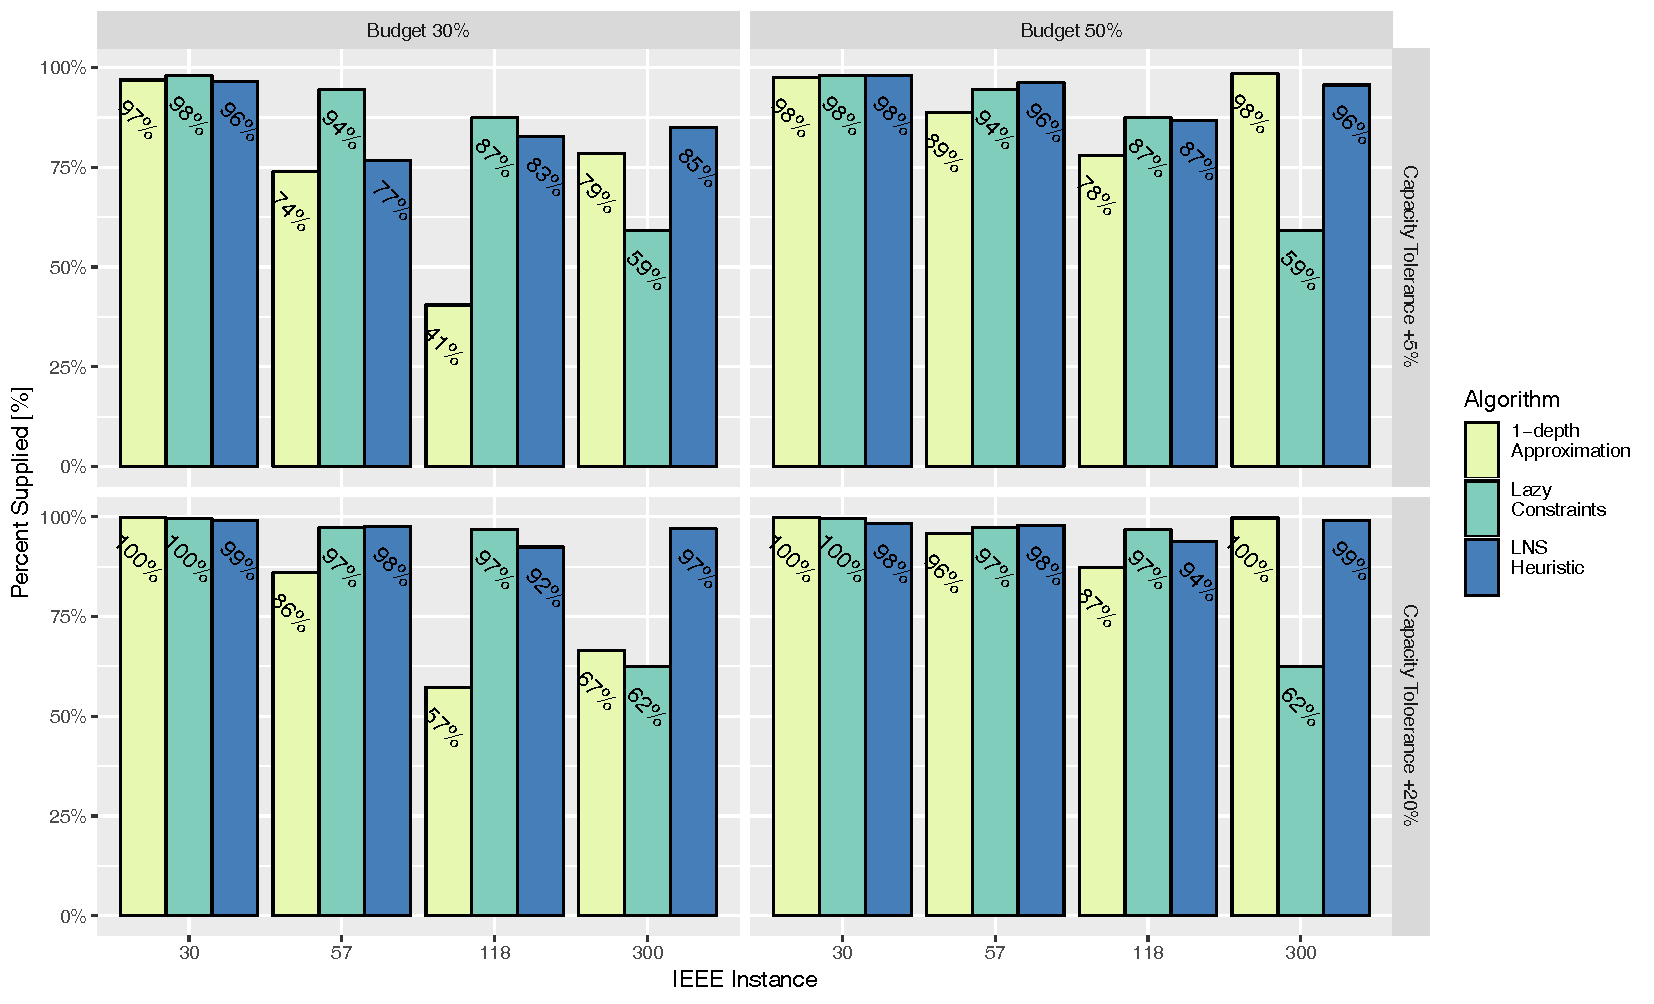
\includegraphics[width=0.8\textwidth]{Aux_files/12hour_instance_results.pdf}
\end{figure}
\end{frame}
\begin{frame}
\frametitle{Results (2) -- average percent supplied}
\begin{table}%
\center
\scriptsize
\begin{tabular}{lccccc}
 & \multicolumn{4}{c}{Percent Supplied Average [\%]} & Overall\\
Algorithm & IEEE30 & IEEE57 & IEEE118 & IEEE300 & Average [\%]\\ \toprule
Lazy Constraints & 98.8 & 95.9 & 92.1 & 60.8 & 86.9\\ \midrule
LNS Heuristic & 98.0 & 92.1 & 89.0 & 94.2 & 93.3\\ \midrule
1-depth Approximation & 98.5 & 86.1 & 65.8 & 85.8 & 84.1 \\ \bottomrule
\end{tabular}
\end{table}
\end{frame}


\section{Conclusions}
\subsection{Conclusions}
\begin{frame}
\frametitle{Conclusions}
\begin{itemize}
	\item A characterization of power grids with 1-depth cascade.\pause
	\item Expected supplied power as a measure for quantifying robustness.\pause
	\item A new method to combine investment decisions with the cascade phenomena. Three robustness optimization algorithms:
	\begin{itemize}
		\item LNS Heuristic.
		\item 1-depth approximation.
		\item Lazy constraints.
	\end{itemize}\pause
	\item Performance vary, depending on instance type, but 1-depth tends to under perform, LNS seems to yield very good solution in most cases.\pause
	\item Further research: generalize the 1-depth characterization, improve tractability of lazy constraint method, tighter upper bounds on solutions.\pause
\end{itemize}
How about ``timely'' considerations? (year + daily variations)
\begin{itemize}
	\item Sarid, A., and Tzur, M., ``The multi-scale generation and transmission expansion model.'', \emph{Energy}, 148 (2018): 977-991.
\end{itemize}
\end{frame}

\subsubsection{Get in Touch}
\begin{frame}
\LARGE Thank you\\
\vspace{2.5cm}
\normalsize
Adi Sarid\\
adi@sarid-ins.co.il
\end{frame}

\section{Multiscale}
\begin{frame}
\frametitle{The ``intricacies'' of time}
So far we haven't treated the intricacies of time:
\begin{itemize}
	\item How to perform the expansion plan over time (years).
	\item How to consider the different times of days (and seasons).
\end{itemize}
\centering
\includegraphics<1>[width=0.5\textwidth]{Aux_files/demand_private.png}
\includegraphics<2>[width=0.5\textwidth]{Aux_files/ev_naive.png}
\includegraphics<3>[width=0.5\textwidth]{Aux_files/smart.png}
\includegraphics<4>[width=0.5\textwidth]{Aux_files/dg.png}
\end{frame}

\begin{frame}
\frametitle{Multiscale model} % Fix here to have a title...
\centering
\vspace{-0.25in}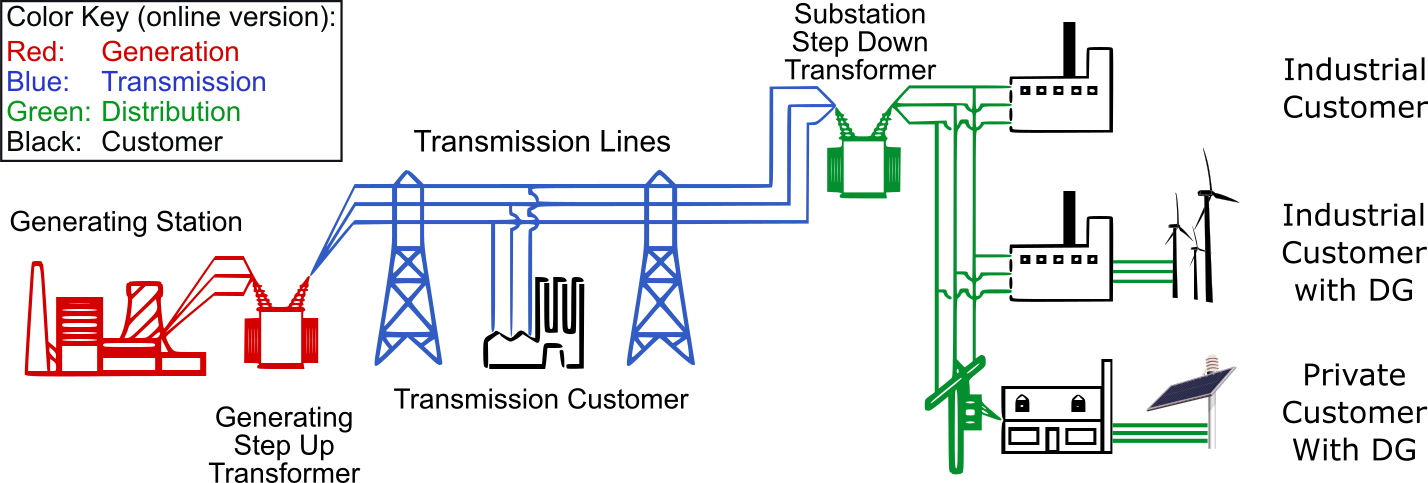
\includegraphics[width=.3\textwidth]{Aux_files/figure_1_Electricity_grid_simple_North_America.png}\vspace{0.1in}\\
%\flushleft
\tiny
\begin{tabular}{lp{2.5cm}p{2.5cm}p{2cm}}
					& \textcolor{adired}{Generation facilities} & \textcolor{adiblue}{Transmission} & \textcolor{adigreen}{Consumers}\\
            		& \textcolor{adired}{(power stations)} & \textcolor{adiblue}{(substations and lines)} & \textcolor{adigreen}{(distribution)}\\\toprule\pause
Establish/upgrade 	& Main generation facilities' capacity (when and where)  & Substation capacity and transmission lines (when and where) & - \\\midrule\pause
Flow problem		& Generation of electricity				& Flow equations & Satisfy demand\\\midrule\pause
Integer variables	& $Z^y_i(m)$ & $Z^y_i(m)$, $X_{ij}^y(m)$ & - \\
					& $U_i^y(m_1,m_2)$ & $U_i^y(m_1,m_2)$, $R^y_{ij}(m_1,m_2)$ & -\\\midrule\pause
Continuous variables & $W_{it}^y$ & $Y^y_{ijt}$ & $W_{it}^y$ \quad (DG) \\\midrule\pause
                    & Parameters: & & \\\midrule
Processing capacity & - & $p_i(m)$, $l_{ij}(m)$ & demand $d_{it}^y$\\\midrule\pause
Generation capacity & $k_{it}(m)$ & - & $k_{it}$ \\
		            & & & $w_{it}$ (unavoidable output) \\\midrule\pause
Installation costs  & $f_i^y(m_1,m_2)$ & $f_i^y(m_1,m_2)$, $c_{ij}^y(m_1,m_2)$ & -\\\bottomrule
\end{tabular}\pause
\flushleft
Additional parameters: $h_{it}$ generation cost, $\tau_t$ length of time interval $t$, $\delta_{ij}, \gamma_i$ energy loss coefficients
\end{frame}

\begin{frame}
\frametitle{The objective}	
Minimize overall costs of installations, upgrades and operating:\scriptsize
\begin{align}
\min{\sum_{y\in\mathcal{Y}}\left(\sum_{i\in\NN}{\sum_{m_1<m_2}f_i^y(m_1,m_2)U_i^y(m_1,m_2)} + \sum_{(i,j)\in\mathcal{L}}\sum_{m_1<m_2}c_{ij}^y(m_1,m_2)R^y_{ij}(m_1,m_2) \right)\notag}\\
+ \sum_{y\in\mathcal{Y}}\sum_{i\in\NN_g}\sum_{t\in\mathcal{T}}\tau_th_{it}^yW_{it}^y\label{FND:objective}
\end{align}
\end{frame}

\begin{frame}
% * <adisarid@gmail.com> 2016-05-04T07:06:41.313Z:
%
% Skip ahead here, by saying most are standard constraints.
%
% ^.
\small Conservation of flow: \tiny
\begin{align}
& \sum_{j\in\NN}{Y^y_{jit}} - d^y_{it} + W^y_{it} = \sum_{j\in\NN}Y^y_{ijt} & \label{FND:flow} \forall i\in\NN, t\in\mathcal{T}, y\in\mathcal{Y}\\
& \sum_{j\in\NN_{sg}}{Y^y_{jit}} + W^y_{it} \geq \sum_{j\in\NN_{sg}}Y^y_{ijt} & \label{FND:high_volt} \forall i\in\NN_{sg}, t\in\mathcal{T}, y\in\mathcal{Y}
\end{align}
% {\color{red}\begin{align}
% \theta_{jty}^y-\theta_{ity}^y-x_{ji}(m)Y^y_{jit}=0 & \hspace{1in}\qquad\label{FND:voltage} \forall i,j\in\NN, t\in\mathcal{T}, y\in\mathcal{Y}
% \end{align}}
\small Processing capacity: \tiny
\begin{align}
	 & \sum_{\{i,j\}\notin\NN_{sg}}{Y^y_{ijt}} \leq \sum_{m=1}^{M_i}p_i(m)Z^y_i(m), & \label{FND:process_capacity} \forall i\in\NN, t\in\mathcal{T}, y\in\mathcal{Y}
\end{align}
\small Manufacturing capacity: \tiny
\begin{align}
	 & W^y_{it}\leq \sum_{m=1}^{M_i}{k_{it}(m)Z^y_i(m)}, \label{FND:establish_facility} &\forall i\in\NN_g, t\in\mathcal{T}, y\in\mathcal{Y}\\
	 & W^y_{it}\geq \sum_{m=1}^{M_i}{w_{it}(m)Z^y_i(m)}, \label{FND:min_generation} &\forall i\in\NN_g, t\in\mathcal{T}, y\in\mathcal{Y}
\end{align}

\end{frame}

\begin{frame}
	\scriptsize 	Link's flow capacity: \tiny
\begin{align}
	 & Y^y_{ijt}\leq \sum_{m=0}^{M_{ij}}{l_{ij}(m)X^y_{ij}(m)}, \label{FND:link_installed} &\forall (i,j)\in\mathcal{L}, t\in\mathcal{T}, y\in\mathcal{Y}
\end{align}
\scriptsize Substation's capacity state and upgrade: \tiny
\begin{align}
	& \sum_{m=0}^{M_i}{Z_i^y(m)}=1, \label{FND:certain_level} &\forall i\in \NN, y\in\mathcal{Y}\\
	& \sum_{m=1}^{M_i}mZ_i^y(m)=\sum_{m=1}^{M_i}mZ_i^{y-1}(m)+\sum_{m_1<m_2}(m_2-m_1)U_i^y(m_1,m_2), & \notag\\
	&  \label{FND:node_upgrade} & \forall i\in\NN, y\in\mathcal{Y}
\end{align}

\scriptsize Upgrade of nodes definition: \tiny
\begin{align}
  & \sum_{m_2: m_2>m_1}U_i^y(m_1,m_2)\leq Z_i^{y-1}(m_1), \label{FND:upgrade_mat} & \forall i \in\NN, y\in\mathcal{Y}, 0\leq m_1<M_i
\end{align}
	
\end{frame}

\begin{frame}
\scriptsize Establishment and upgrade of transmission lines: \tiny
\begin{align}
	\sum_{m=1}^{M_{ij}}X_{ij}^y(m)\leq 1-Z^y_i(0) \label{FND:link_then_facility}, & \hspace{2in}\forall (i,j)\in\mathcal{L}, i\in \NN_g, y\in\mathcal{Y} %\symbol{92}\mathcal{L}_s
\end{align}

\begin{align}
	& \sum_{m=1}^{M_{ij}}mX_{ij}^y(m)=\sum_{m=1}^{M_{ij}}mX_{ij}^{y-1}(m)+\sum_{m_1<m_2}(m_2-m_1)R_{ij}^y(m_1,m_2), & \notag \\
	& \hspace{2.9in} \forall (i,j)\in\mathcal{L}, i\in\NN, y\in\mathcal{Y} \label{FND:link_up} &
\end{align}
\begin{align}
  & \sum_{m_2: m_2>m_1}R_{ij}^y(m_1,m_2)\leq X_{ij}^{y-1}(m_1), & \notag\\
	& \hspace{1.9in} \forall (i,j)\in\mathcal{L}, i \in\NN, y\in\mathcal{Y}, 0\leq m_1<M_{ij} \label{FND:link_up2} & 
\end{align}
\begin{align}
  %& {\sum_{m_1<m_2}{R_{ij}^y(m_1,m_2)}}\leq 1, \label{FND:upgrade_once} & \forall (i,j)\in\mathcal{L}, i\in\NN, y\in\mathcal{Y}\\ % redundant due to next constraint
	& X^y_{ij} = X^y_{ji} , \label{FND:edge_symm} &\forall (i,j)\in\mathcal{L}, y\in\mathcal{Y} %\symbol{92}\mathcal{L}_s
\end{align}
\end{frame}

\begin{frame}
\small Decision variables' range: \tiny
\begin{align}
	 & Z^y_i(m) \in \{0,1\}, \label{FND:Z_int} &\forall i\in\NN, y\in\mathcal{Y}\\
	 & X^y_{ij}(m) \in \{0,1\}, &\forall (i,j)\in\mathcal{L}, i\in\NN, y\in\mathcal{Y}\\
	 & U_i^y(m_1, m_2)\in\{0,1\}, & \forall i\in\NN, y\in\mathcal{Y}\\
	 & R_{ij}^y(m_1, m_2)\in\{0,1\}, & \forall (i,j)\in\mathcal{L}, y\in\mathcal{Y}\\
	 & Y^y_{ijt}\geq0, &\forall (i,j)\in\mathcal{L}, t\in\mathcal{T}, y\in\mathcal{Y}\\
	 & W^y_{ijt}\geq0, \label{FND:W_pos} &\forall (i,j)\in\mathcal{L}, t\in\mathcal{T}, y\in\mathcal{Y}
\end{align}

\quad \\ \quad \\ \small
\onslide<2>{The addition of energy loss requires modification of the objective function and some of the earlier constraints.}
\end{frame}

\begin{frame}
\frametitle{Numerical experiments -- Small instances (33 nodes)}
\framesubtitle{Distributed generation}
\begin{table}[htbp]
\tiny
  \centering
	\begin{tabular}{l|l|c|c|c|c|c|c}
    \hline
    & &       & \textbf{Substation} & \textbf{Line} & \textbf{Gen. facilities} & \textbf{Total} & \textbf{Gen.} \\
    \# & \textbf{Name} & \textbf{Obj.} & \textbf{Costs} & \textbf{Costs} & \textbf{Costs} & \textbf{Invest.} & \textbf{Costs} \\ \hline
    1 & \textbf{Base} & 350.2 & 25    & 47.09 & 165   & 237.1 & 113.1 \\ \hline
    2 & \textbf{DG 5\%} & 327.3 & 25    & 43.38 & 165   & 233.4 & 93.94 \\
    3 & \textbf{DG 10\%} & 308.1 & 25    & 43.38 & 165   & 233.4 & 74.73 \\
    \hline
    \end{tabular}%
    %\label{tab:ResSmallInstances}%
	%\caption{Comparison of small instances (33 nodes)}
\end{table}%
\normalsize
\begin{block}{Interesting observations}
\onslide<2->{Introduction of 5-10\% DG nodes ($\sim$17-34\% production by DG) yielded similar infrastructure investments -- same facilities, decreased line investments\\}
\onslide<3->{Total costs decreased by $\sim$7-12\%\\}
\onslide<4->{No feasible solution above 10\% DG nodes -- excess quantity above transmission capacity + not enough neighborhood demand}
\end{block}
\end{frame}


\begin{frame}
\frametitle{Numerical experiments -- Small instances (33 nodes)}
\framesubtitle{Electric vehicles}
\begin{table}[htbp]
\tiny
  \centering
	\begin{tabular}{l|l|c|c|c|c|c|c}
    \hline
    & &       & \textbf{Substation} & \textbf{Line} & \textbf{Gen. facilities} & \textbf{Total} & \textbf{Gen.} \\
    \# & \textbf{Name} & \textbf{Obj.} & \textbf{Costs} & \textbf{Costs} & \textbf{Costs} & \textbf{Invest.} & \textbf{Costs} \\ \hline
    1 & \textbf{Base} & 350.2 & 25    & 47.09 & 165   & 237.1 & 113.1 \\ \hline
    \textcolor<2>{orange}{4} & \textbf{EV sm40\%} & 364.5 & 25    & 47.09 & 165   & 237.1 & 127.4 \\
    \textcolor<3>{orange}{5} & \textbf{EV na\"{i}10\% + sm40\%} & 392.1 & 25    & 51.14 & 185 & 261.1 & 131 \\ \hline
    \textcolor<3>{orange}{6} & \textbf{EV na\"{i}-sl10\%} & 358.1 & 29 & 47.43 & 165   & 241.4 & 116.6 \\
    \textcolor<3>{orange}{7} & \textbf{EV na\"{i}-sl20\%} & 382.1 & 25    & 51.86 & 185 & 261.9 & 120.3 \\
    \textcolor<3>{orange}{8} & \textbf{EV na\"{i}-sl10\%+sm40\%} & 372.3 & 29 & 47.43 & 165   & 241.4 & 130.9 \\
    \textcolor<3>{orange}{9} & \textbf{EV na\"{i}-sl20\%+sm40\%} & 396.4 & 25    & 51.86 & 185 & 261.9 & 134.6 \\ \hline
    \textcolor<2>{orange}{10} & \textbf{EV sm-noon10\%} & 353.8 & 25    & 47.1  & 165   & 237.1 & 116.7 \\
    \textcolor<2>{orange}{11} & \textbf{EV sm-noon30\%} & 365.6 & 29 & 47.68 & 165   & 241.7 & 123.9 \\
    \textcolor<2>{orange}{12} & \textbf{EV sm-noon50\%} & 398.8 & 29 & 53.87 & 185 & 267.9 & 130.9 \\
    \hline
    \end{tabular}%
  %\label{tab:ResSmallInstances}%
	%\caption{Comparison of small instances (33 nodes)}
\end{table}%
\footnotesize
\begin{block}{Interesting observations}
\onslide<2->{Smart consumers -- didn't affect much on the infrastructure\\}
\onslide<3->{Na\"ive consumers -- depending on penetration level, required more infrastructure investments\\}
\onslide<4->{Max EV penetration level depends on demand patterns\\(smart - up to 80\% versus na\"ive up to 10\%)}
\end{block}
\end{frame}

\end{document}

